\subsection{Kandidatensuche}\label{sec:kandidatensuche}
Die Kandidatensuche, im Folgenden Suche genannt, wird über eine klassische Graphensuche durchgeführt, wobei der vollständige
Graph alle möglichen Stösse enthält.
Für die Suche gibt es zwei Möglichkeiten, entweder wird bei der weissen Kugel gestartet und von dort ein Stoss gesucht,
welcher eine andere Kugel ins Loch spielt, oder es wird bei einem oder mehreren Löchern gestartet und von dort ein Stoss gesucht,
welcher von der weissen Kugel ausgehend eine andere Kugel ins Loch spielt.

Nachfolgend wird die Rückwärtssuche beschrieben, welche ausgehend vom Zielloch startet, eine einzulochende Kugel findet
und anschliessend den Stoss bis zur weissen Kugel zurück sucht.
Dementsprechend ist der Root-Knoten des Suchbaumes das zu treffende Ziel (Loch).
Da ein handelsüblicher Billardtisch mehrere Löcher hat, muss pro Loch eine separate Suche durchgeführt werden.

Bei der Durchführung eines Expansionsschrittes werden ausgehend von einem Knoten im Suchbaum dessen Nachfolger-Knoten ermittelt.
Diese stellen im Fall vom Root-Knoten Kugeln dar, welche in dieses Loch gespielt werden könnten.
Aus diesen Kugeln werden Kugel-Knoten gebildet, welche diese Kugeln entweder auf direktem Wege oder indirekt über die Bande
in das Loch spielen lassen sollen.
Von diesen Kugel-Knoten startend, werden deren Nachfolger-Knoten in weiteren Expansionsschritten ermittelt, welche
wiederum Kugel-Knoten darstellen.
Diese Kugel-Knoten stellen dann Kugeln dar, welche die Kugel des Vorgänger-Kugel-Knotens entweder auf direktem Wege oder indirekt
über die Bande treffen sollen.
Sofern ein Kugel-Knoten die weisse Kugel darstellt, so ist dieser Kugel-Knoten ein Endzustand und damit ist der Stoss
über die Kette von Nachfolger- zu Vorgänger-Kugel-Knoten definiert.

\newpage
Zur Veranschaulichung des Prinzips folgt ein Beispiel. Es wird vereinfacht angenommen,
dass der Tisch nur ein Loch hat. Für mehrere Ziele ergeben sich mehrere Suchbäume, einen pro Loch.
In Abbildung \ref{fig:backwardsearch_1} erfolgt die Eingabe des Suchalgorithmus in Form des Root-Knotens.
Es wird nur das zu treffende Ziel definiert.

\begin{figure}[h!]
    \begin{center}
        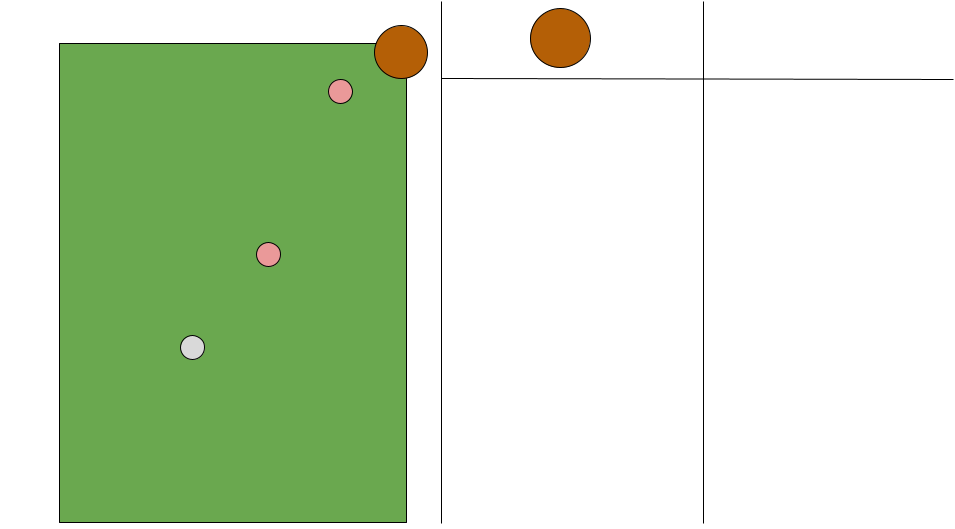
\includegraphics[width=0.5\linewidth]{../common/03_billiard_ai/resources/11_backwardsearch_1.png}
    \end{center}
    \caption{Kandidatensuche 1: Links ist der Spielstand auf dem Billardtisch abgebildet. Auf der rechten Seite des Tisches ist der Suchbaum dargestellt.
    Im ersten Schritt wurden ausgehend vom Zielloch noch keine Kugeln expandiert.
    Es stehen die beiden roten Kugeln zur Auswahl.}
    \label{fig:backwardsearch_1}
\end{figure}

In einem zweiten Schritt wird die einzulochende Kugel definiert. Es kommen lediglich die beiden roten Kugeln in Frage.
Nachfolgend wird der Pfad weiter betrachtet, bei dem die beim Loch näherstehende rote Kugel, gewählt wurde.
Abbildung \ref{fig:backwardsearch_2} zeigt, dass der Suchbaum um einen Knoten erweitert wurde.
\begin{figure}[h!]
    \begin{center}
        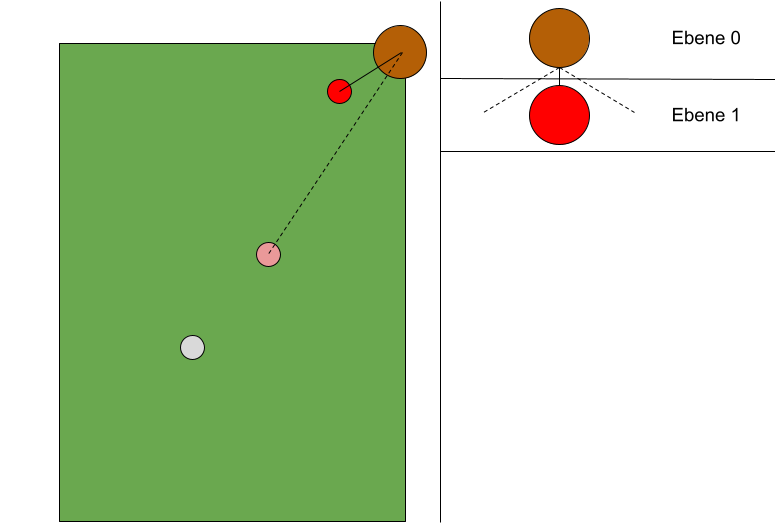
\includegraphics[width=0.5\linewidth]{../common/03_billiard_ai/resources/12_backwardsearch_2.png}
    \end{center}
    \caption{Kandidatensuche 2: Im ersten Expansionsschritt wurde die dunkelrot eingefärbte Kugel als einzulochende Kugel gewählt.
    Im Suchbaum ist diese dadurch als Knoten eingefügt worden. }
    \label{fig:backwardsearch_2}
\end{figure}

In Abbildung \ref{fig:backwardsearch_3} erfolgt der letzte Schritt. Hier sind verschiedene Optionen möglich, bspw.
könnte die weisse Kugel direkt oder über die Bande an die zuvor gewählte rote Kugel gespielt werden. Es könnte aber auch
die andere rote Kugel an die zuvor gewählte rote Kugel gespielt werden. Hier wird der Fall betrachtet, dass die weisse Kugel
indirekt über eine Bande an die zuvor gewählte rote Kugel gespielt wird.
\begin{figure}[h!]
    \begin{center}
        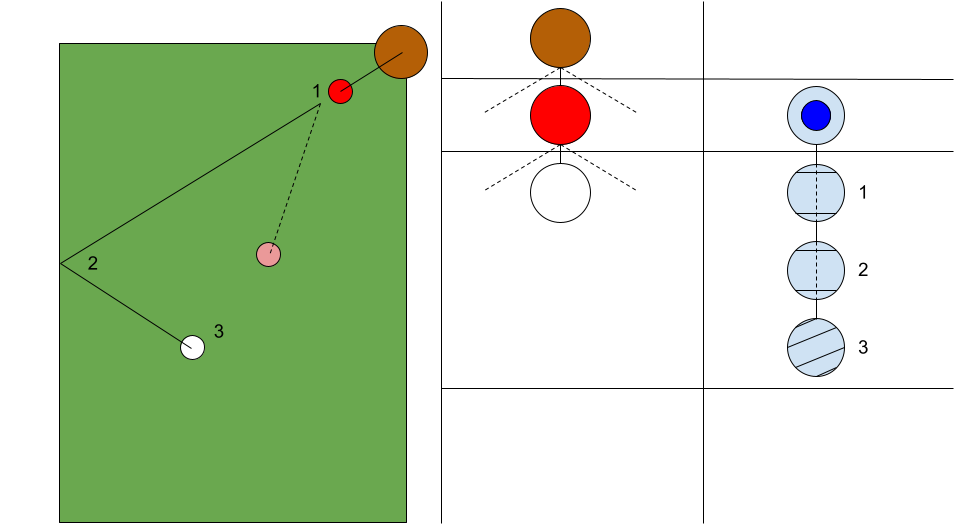
\includegraphics[width=0.5\linewidth]{../common/03_billiard_ai/resources/13_backwardsearch_3.png}
    \end{center}
    \caption{Kandidatensuche 3: Im letzten Expansionsschritt wurde die weisse Kugel gewählt und wird über die Bande an die rote Kugel gespielt.
    Der Suchbaum hat demnach einen neuen Knoten für die weisse Kugel, wodurch ein Pfad für einen vollständiger Stoss entstanden ist.}
    \label{fig:backwardsearch_3}
\end{figure}

\newpage
Algorithmus \ref{alg:backward_search} verdeutlicht den Ablauf der \glqq Expand-Funktion\grqq. Zuerst wird eine
leere Liste namens \glqq nodes\grqq{} angelegt. Diese wird danach mit Nodes gefüllt, welche entweder durch einen Stoss
über eine weitere Kugel oder indirekt über die Bande zustande kommen. Die Nodes bilden das Ergebnis der Funktion.

\begin{algorithm}[H]
    \DontPrintSemicolon
    \SetKwFunction{expand}{expand}
    \SetKwProg{Fn}{Function}{}{}
    \Fn{\expand{node: Node, constantObjects: list} $\longrightarrow$ list[Node]}{
        nodes $\longleftarrow$ list()\\
        nodes $\longleftarrow$ append(expandBalls(node, constantObjects), nodes)\\
        nodes $\longleftarrow$ append(expandBank(node, constantObjects), nodes)\\
        \KwRet nodes
    }
    \caption{Algorithmus zur Durchführung eines Expansionsschritts bei der Kandidatensuche}
    \label{alg:backward_search}
\end{algorithm}

\subsubsection{Expansion einer Kugel}
In der anzuwendenden Graphensuche müssen die nächsten Knoten expandiert werden.
Eine Expansion kann über eine Kugel- oder über eine Bandenkollision stattfinden.

\paragraph{Expansion über eine Kugelkollision}\mbox{}\\

Bei einer Expansion einer Kugel wird der nächste Zielpunkt berechnet.
Das Prinzip wird in Abbildung \ref{fig:kugelexpansion} veranschaulicht.
Der Zielpunkt $T$, wohin die Kugel gespielt werden soll, ist bekannt.
Weiterhin ist die aktuelle Position $S$ der Kugel bekannt. Dazwischen kann der Vektor $\vec{d}$ gebildet werden.
\begin{align}
    \vec{d} = S - T
\end{align}
Damit die Kugel in Richtung des Zielpunkts $T$ rollt, muss diese von einer anderen Kugel am Punkt $Z$ angestossen werden.
Daher gilt es $Z$ zu bestimmen.
Der neue Zielpunkt $Z$ wird mithilfe des Vektors $d$ und dem bekannten Kugelradius $r$ berechnet.
\begin{align}
    Z = S + 2 \cdot r \cdot \hat{d}
\end{align}

\begin{figure}[h!]
    \begin{center}
        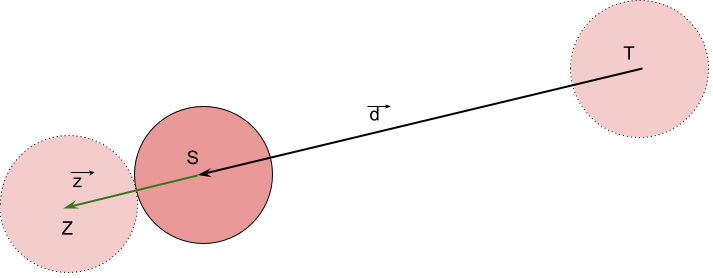
\includegraphics[width=0.5\linewidth]{../common/03_billiard_ai/resources/35_suchkandidat_kugel_expand.png}
    \end{center}
    \caption{Kugelexpansion}
    \label{fig:kugelexpansion}
\end{figure}

\paragraph{Expansion über eine Bandenkollision}\label{kandidatensuche:bandenkollisionstheorie}\mbox{}\\

Eine Kugel kann ebenso über eine oder mehrere Banden expandiert werden. Dazu muss bekannt sein, wie der Verlauf einer
Kugel nach einer Bandenkollision aussieht. Um diese Frage beantworten zu können, wurden zwei Arbeiten betrachtet.
Nach diesen Quellen gilt für den Stoss einer Kugel über die Bande, dass im Falle eines nicht vorhandenen Spins
der Ausfallswinkel dem Einfallswinkel entspricht. Dieses Verhalten wurde von den Autoren des Papers \glqq A theoretical analysis of billiard ball dynamics under cushion impacts\grqq{}
untersucht \cite{10.1243/09544062JMES1964}.
Der Abschnitt \glqq b\grqq{} der Abbildung \ref{fig:rail_rebound_angle_no_spin} zeigt die
funktionale fast lineare Abhängigkeit des Ausfallswinkels vom Einfallswinkel.
Diese Werte wurden anhand verschiedener Geschwindigkeiten in praktischen Experimenten ermittelt \cite{10.1243/09544062JMES1964}.

\begin{figure}[h!]
    \begin{center}
        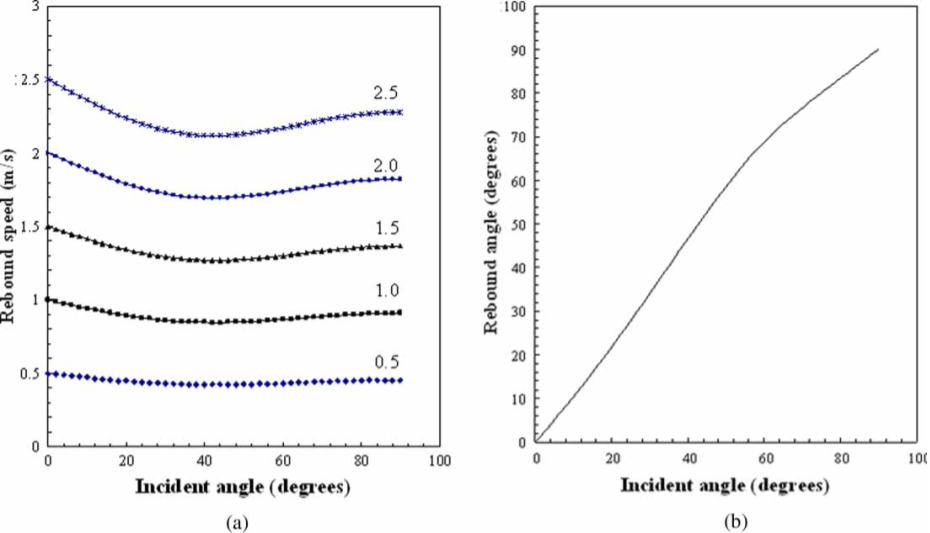
\includegraphics[width=0.5\linewidth]{../common/03_billiard_ai/resources/55_rail_rebound_angle_no_spin.png}
    \end{center}
    \caption{Geschwindigkeits- und Ausfallswinkelabhängigkeiten zum Einfallswinkel einer Kugel ohne Spin an einer Bande.
    Entnommen aus der Arbeit \cite{10.1243/09544062JMES1964} des Kapitels \glqq Results and Discussion\grqq. }
    \label{fig:rail_rebound_angle_no_spin}
\end{figure}

\newpage
Eine weitere Bestätigung und eine ebenso ausführliche Behandlung des Themas findet sich im Buch \glqq The illustrated principles
of pool and billiards\grqq. Auch dieser Arbeit liegen praktische
\href{https://billiards.colostate.edu/high-speed-video/}{Experimente} zugrunde, die die Theorie bestätigen.
Grundsätzlich gilt das Prinzip 6.1 \glqq Bank shot geometry\grqq, welches besagt, dass
der Ausfallswinkel dem Einfallswinkel entspricht, dies ist
jedoch bei schwachen und starken wie auch bei Stössen der Bande sehr nahe liegenden Kugeln nicht korrekt \cite{book:the_ilustrated_principles_of_pool_and_billiards}.
So besagt das Prinzip 6.6 \glqq Rail throwback at high speed\grqq, dass der Ausfallswinkel kleiner wird, je stärker der Stoss ausgeführt wird.
Dieser Effekt tritt vor allem bei Einfallswinkeln zwischen $20^{\circ}$ und $50^{\circ}$ auf und ist auf
die seitliche Kompression der Bande zurückzuführen. Diese wird unterschiedlich stark eingedrückt und gibt durch die
darauffolgende Entspannung eine stärkere Kraft in die einfallende Richtung der Kugel zurück \cite{book:the_ilustrated_principles_of_pool_and_billiards}.
Dieser Umstand wird in der Abbildung \ref{fig:rebound_angle_no_spin_fast_shot} gezeigt.

\begin{figure}[h!]
    \begin{center}
        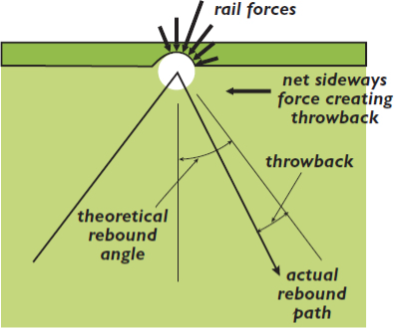
\includegraphics[width=0.3\linewidth]{../common/03_billiard_ai/resources/56_rebound_angle_no_spin_fast_shot.png}
    \end{center}
    \caption{Unterschiedliche Belastung der Bande bei starkem Stoss einer Kugel.
    Entnommen aus dem Buch \cite{book:the_ilustrated_principles_of_pool_and_billiards} des Kapitels \glqq 6 Bank and kick shots\grqq.}
    \label{fig:rebound_angle_no_spin_fast_shot}
\end{figure}

Trifft die Kugel langsam auf die Bande auf, so gilt Prinzip 6.7 \glqq Curved rebound path due to slow-speed roll\grqq.
Dieses verweist auf den Umstand, dass eine Kugel, die langsam auf die Bande trifft, aufgrund des resultierenden
Topspins kurvenförmig wegrollt. Der Effekt ist bei einem Einfallswinkel von $45^{\circ}$ am stärksten \cite{book:the_ilustrated_principles_of_pool_and_billiards}.
Die Abbildung \ref{fig:rebound_angle_no_spin_slow_shot} verdeutlicht das Prinzip.

\begin{figure}[h!]
    \begin{center}
        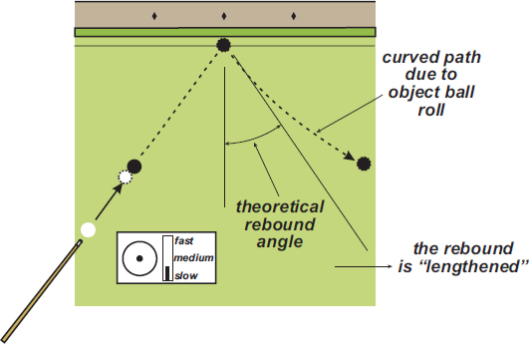
\includegraphics[width=0.4\linewidth]{../common/03_billiard_ai/resources/57_rebound_angle_no_spin_slow_shot.png}
    \end{center}
    \caption{Einfluss des Topspins auf den Ausfallswinkel bei schwachem Stoss einer Kugel an eine Bande.
    Entnommen aus dem Buch \cite{book:the_ilustrated_principles_of_pool_and_billiards} des Kapitels \glqq 6 Bank and kick shots\grqq.}
    \label{fig:rebound_angle_no_spin_slow_shot}
\end{figure}

Trifft eine Kugel langsam auf die Bande auf und ist sehr nahe, so dass sie zum Zeitpunkt der Kollision noch nicht zu rollen begonnen hat,
gilt Prinzip 6.8 \glqq Smaller rebound angle when close to the rail\grqq.
Dieses besagt, dass der Ausfallswinkel demnach kleiner wird \cite{book:the_ilustrated_principles_of_pool_and_billiards}.
Der resultierende Unterschied aufgrund der Distanzen wird in Abbildung \ref{fig:rebound_angle_no_spin_slow_shot_distance} veranschaulicht.

\begin{figure}[h!]
    \begin{center}
        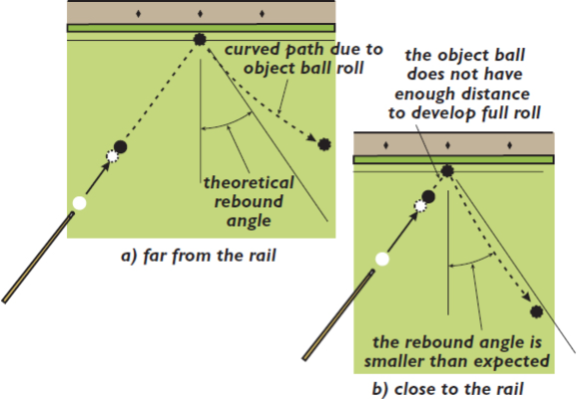
\includegraphics[width=0.4\linewidth]{../common/03_billiard_ai/resources/58_rebound_angle_no_spin_slow_shot_distance.png}
    \end{center}
    \caption{Einfluss der Distanz auf den Ausfallswinkel bei schwachem Stoss einer Kugel an eine Bande.
    Entnommen aus dem Buch \cite{book:the_ilustrated_principles_of_pool_and_billiards} des Kapitels \glqq 6 Bank and kick shots\grqq.}
    \label{fig:rebound_angle_no_spin_slow_shot_distance}
\end{figure}

\newpage
Aufgrund dieser Erkenntnisse und der gegebenen Abhängigkeit wird der Ausfallswinkel dem Einfallswinkel gleichgesetzt.
Technisch geschieht dies über einen geometrischen Ansatz durch eine Spiegelung \cite{math.stackexchange:1}
des Zielpunkts an der entsprechenden Bande, über welche gespielt werden soll.
In Abbildung \ref{fig:Tiefe über Bande erreichen mittels Reflektion} wird ein Suchschritt über eine Bande visualisiert.
Es wird ein Punkt $A$ an einer Bande gesucht, zu welchem die Kugel $B$ gespielt werden muss, um die Kugel $C$ zu treffen.
Dieser Bandenkollisionspunkt $A$ wird mithilfe eines Spiegelpunkts $\bar{C}$ des Punktes $C$ an der Bande berechnet.

\begin{figure}[h!]
    \begin{center}
        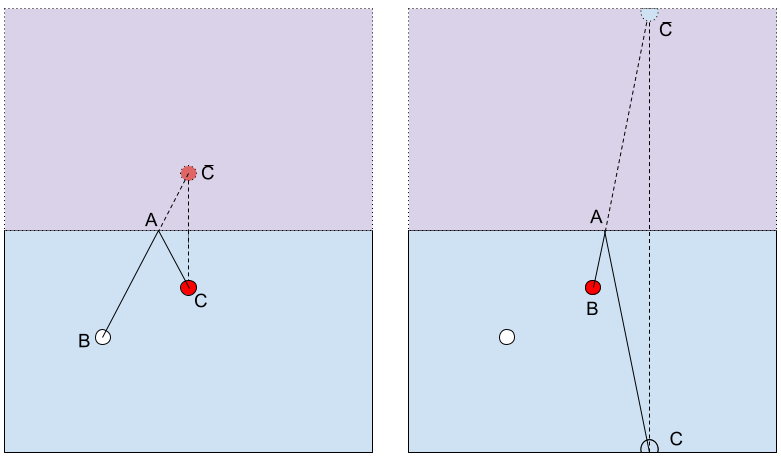
\includegraphics[width=0.5\linewidth]{../common/03_billiard_ai/resources/47_rail_reflection_1.png}
    \end{center}
    \caption{Zwei Fälle für ein Bandenspiel:
    Im ersten Fall wird für die weisse Kugel ein Kollisionspunkt an der oberen Bande bestimmt, um die rote Kugel zu treffen.
    Im zweiten Fall wird für die rote Kugel ein Kollisionspunkt an der oberen Bande bestimmt, um ins Ziel zu treffen.
    }
    \label{fig:Tiefe über Bande erreichen mittels Reflektion}
\end{figure}

Gegeben sind die folgenden Angaben (Parameter werden grossgeschrieben, Variablen dagegen klein):
\begin{align}
    B = \begin{pmatrix}B_X\\B_Y\end{pmatrix},
    C = \begin{pmatrix}C_X\\C_Y\end{pmatrix},
    \bar{C} = \begin{pmatrix}\bar{C_X}\\\bar{C_Y}\end{pmatrix},
\end{align}
Der Schnittpunkt kann über zwei Geraden berechnet werden, die über die Parameterform gegeben sind.
Eine dieser Geraden liefert der gespiegelte Punkt $\bar{C}$ mit $B$.
\begin{align}
    \vec{l} = \vec{\bar{C}} - \vec{B}\\
    L_1 = \vec{B} + \lambda_1 \cdot \vec{l}
\end{align}
Die andere Gerade ist über die Bande (Rail) gegeben, wobei $R_1$ der Startpunkt und $R_2$ der Endpunkt der Bande ist:
\begin{align}
    R_1 = \begin{pmatrix}R_{1X}\\R_{1Y}\end{pmatrix}, R_2 = \begin{pmatrix}R_{2X}\\R_{2Y}\end{pmatrix}\\
    \vec{r} = \vec{R_2} - \vec{R_1}\\
    L_2 = \vec{R_1} + \lambda_2 \cdot \vec{r}
\end{align}
Der Kollisionspunkt $A$ lässt sich über $\lambda_1$ der Gleichung \ref{eq:bandenkollisionspunkt} mithilfe der Linie $L_1$
bestimmen (Herleitung, siehe Anhang \ref{anhang:herleitung:bandenreflektion}).

\begin{align}
    \lambda_1 = \frac{r_x \cdot B_y - r_y \cdot B_x + R_{1,x} \cdot r_y - R_{1,y} \cdot r_x}{l_x \cdot r_y - \cdot l_y \cdot r_x}\label{eq:bandenkollisionspunkt}
\end{align}

Es gilt zu beachten, dass es sich bei der Billardkugel nicht um einen unendlich kleinen Punkt handelt und
daher deren Radius berücksichtigt werden muss.
Das Problem wird in Abbildung ~\ref{fig:bandenreflektion_kugelradius} dargestellt.
\begin{figure}[h]
    \begin{center}
        \includegraphics[width=0.5\linewidth]{../common/03_billiard_ai/resources/48_bandenreflektion_kugelradius.png}
    \end{center}
    \caption{Berücksichtigung des Kugelradius bei Bandenreflektion: Die Bande wird um den Kugelradius in Richtung Tischmitte verschoben.}
    \label{fig:bandenreflektion_kugelradius}
\end{figure}

Einerseits wird als Zielposition $C$ nicht die Kugelposition selbst, sondern ein um den Radius verschobener Punkt in
Gegenrichtung zur gewünschten Laufrichtung $\vec{r}$ der Kugel $C$ definiert. Andererseits wird die Bande, an welcher
gespiegelt wird, um den Radius der Kugel in Richtung des Zentrums verschoben. Die verschobene virtuelle Bande ist grün eingezeichnet.

Durch Studium mehrerer Beispiele wird ein allgemeiner Algorithmus hergeleitet. Hierbei wird das zuvor genannte Problem
mit dem Kugelradius vernachlässigt, da dieses durch die beschriebenen Positionskorrekturen behandelt werden kann.
Der Algorithmus kann unabhängig von dieser Korrektur beschrieben werden.

\newpage
In einem ersten Schritt werden die Banden definiert, über welche der Zielpunkt gespiegelt werden soll. Dies sind in
diesem Beispiel die linke und die obere Bande, dementsprechend werden die grün markierten Spiegel zuerst links und
dann oben angewendet. Es resultieren die Punkte $\bar{C_0}$ und $\bar{C_1}$. Die Abbildung \ref{fig:zweifaches_bandenspiel_a} zeigt die
Situation mitsamt der gespiegelten Punkte.
\begin{figure}[h]
    \begin{center}
        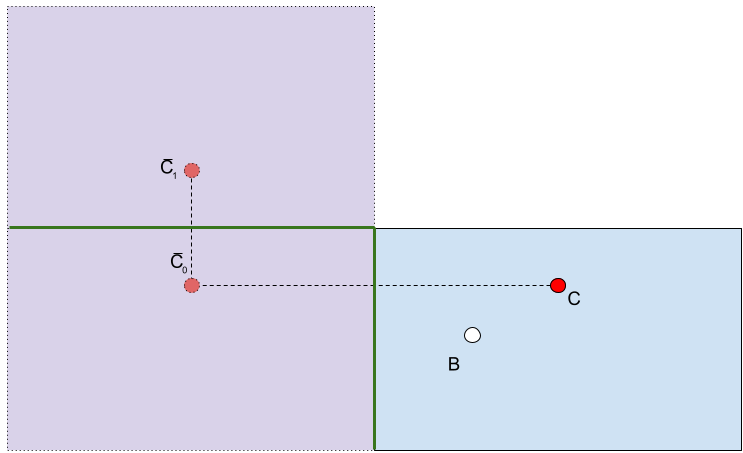
\includegraphics[width=0.5\linewidth]{../common/03_billiard_ai/resources/50_rail_reflection_2_a.png}
    \end{center}
    \caption{Zweifaches Bandenspiel - A: Der Zielpunkt C wurde zuerst an der linken, dann an der oberen Bande gespiegelt.}
    \label{fig:zweifaches_bandenspiel_a}
\end{figure}

Die Abbildung \ref{fig:zweifaches_bandenspiel_b} zeigt das Vorgehen, nachdem die Spiegelungen durchgeführt wurden.
Es wird der letzte Spiegelpunkt $\bar{C_n}$, in diesem Fall $\bar{C_1}$,
beibehalten, die Vorherigen werden verworfen. Vom Startpunkt $B$ aus wird eine Verbindung zum Spiegelpunkt $\bar{C_1}$
gezogen und alle Bandensegmente auf Schnittpunkte geprüft, was schliesslich im Punkt $A_0$ resultiert. Dies ist
der erste Kollisionspunkt mit der Bande und kann der Resultatsmenge hinzugefügt werden. Anschliessend wird der Spiegelpunkt
$\bar{C_1}$ an der Bande gespiegelt, an welcher der Kollisionspunkt liegt, in dem Fall an der Linken. Diese Spiegelung
resultiert im Spiegelpunkt $\bar{C_0}$.
\begin{figure}[h]
    \begin{center}
        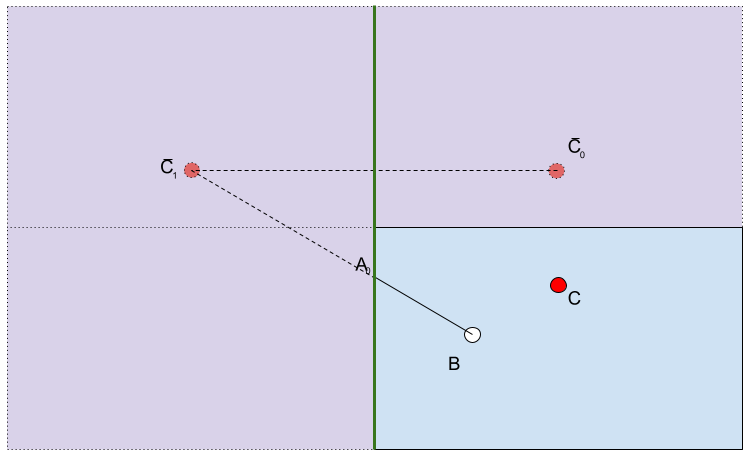
\includegraphics[width=0.5\linewidth]{../common/03_billiard_ai/resources/51_rail_reflection_2_b.png}
    \end{center}
    \caption{Zweifaches Bandenspiel - B: Der Schnittpunkt $A-0$ an der linken Bande ist der erste Bandenkollisionspunkt.
    Um den zweiten Bandenkollisionspunkt zu bestimmen, wird die Spiegelung an der linken Bande rückgängig gemacht.}
    \label{fig:zweifaches_bandenspiel_b}
\end{figure}

\newpage
In der Abbildung \ref{fig:zweifaches_bandenspiel_c} ist der darauffolgende Schritt ersichtlich.
Es gibt zum Vorhergehenden keine wesentlichen Unterschiede.
Es wird wiederum nur der letzte Spiegelpunkt $\bar{C_0}$ beibehalten, zu welchem vom
neuen Startpunkt $A_0$ eine Verbindung gezogen wird.
Diese Halbgerade wird wiederum auf Schnittpunkte mit allen Bandensegmenten geprüft, was im Kollisionspunkt $A_1$ resultiert.
Dieser Kollisionspunkt wird der Resultatsmenge hinzugefügt und der Punkt $\bar{C_0}$
wird an der Bande mit dem Kollisionspunkt gespiegelt, in dem Fall der Oberen.
Diese Spiegelung überführt den Punkt $\bar{C_0}$ auf den ursprünglichen Punkt $C$, was das Ende des Algorithmus
bedeutet.
\begin{figure}[h]
    \begin{center}
        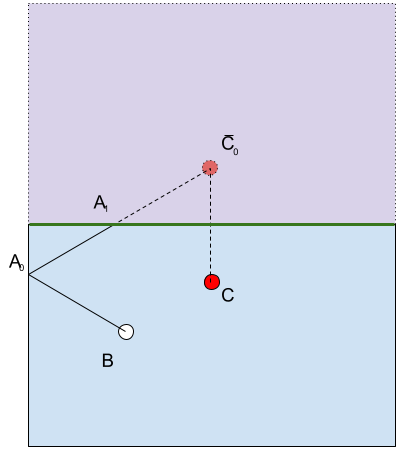
\includegraphics[width=0.5\linewidth]{../common/03_billiard_ai/resources/52_rail_reflection_2_c.png}
    \end{center}
    \caption{Zweifaches Bandenspiel - C: Der Schnittpunkt $A-1$ an der oberen Bande ist der zweite Bandenkollisionspunkt.
    Wenn die Spiegelung an der oberen Bande rückgängig gemacht wird, fällt der Zielpunkt wieder auf den ursprünglichen Punkt C zurück.}
    \label{fig:zweifaches_bandenspiel_c}
\end{figure}

Die Abbildung \ref{fig:zweifaches_bandenspiel_d} zeigt das endgültige Resultat, wenn der letzte Kollisionspunkt $A_1$
mit dem Zielpunkt $C$ verbunden wird.

\begin{figure}[h!]
    \begin{center}
        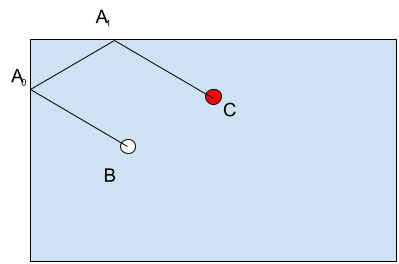
\includegraphics[width=0.5\linewidth]{../common/03_billiard_ai/resources/53_rail_reflection_2_d.png}
    \end{center}
    \caption{Zweifaches Bandenspiel - D: Die weisse Kugel wird von B über $A_0$ und $A_1$ an die rote Kugel an Position C gespielt.}
    \label{fig:zweifaches_bandenspiel_d}
\end{figure}

Dasselbe Prinzip kann auch auf ein Spiel über drei Banden angewendet werden, siehe Abbildung \ref{fig:Dreifache Reflektion an Banden}.
Es wird zuerst an der linken, dann an der oberen und anschliessend an der rechten Bande gespiegelt.
Es wird in einem Schritt wiederum der letzte Spiegelpunkt und dessen Startposition betrachtet, mit welchen der Kollisionspunkt
an einer Bande gefunden werden kann. Danach kann der Spiegelpunkt an dieser Bande gespiegelt werden und der nächste
Schritt kann starten. Dies wird so oft wiederholt, wie es Banden zum Spiegeln hat.
\begin{figure}[h]
    \begin{center}
        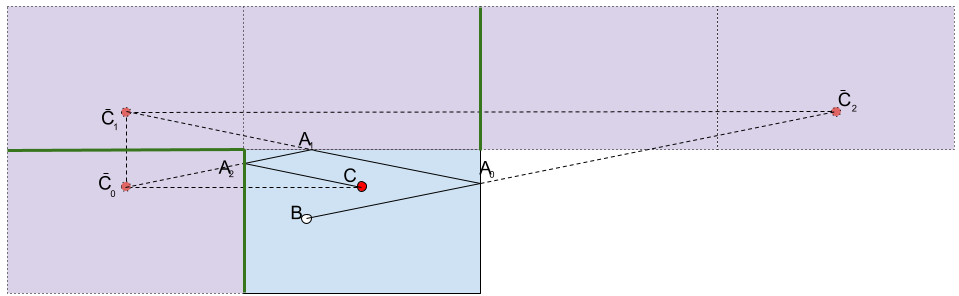
\includegraphics[width=1\linewidth]{../common/03_billiard_ai/resources/54_rail_reflection_3.png}
    \end{center}
    \caption{Dreifache Reflektion an Banden. Es wird zuerst an der linken, dann an der oberen und zuletzt an der rechten Bande gespiegelt.}
    \label{fig:Dreifache Reflektion an Banden}
\end{figure}

Eine Spiegelung kann durch die Anwendung der bandenspezifischen Transformationsmatrix $M$ erzielt werden, wobei $\vec{s}$
für den Spiegelvektor steht (Herleitung, siehe Anhang \ref{anhang:herleitung:bandenreflektion:zielpunkt}).
Hierbei steht der Punkt $C$ für den Zielpunkt, den es zu treffen gilt.
\begin{align}
    M = \begin{pmatrix}s_x & 0 & R^1_x - s_x \cdot R^1_x \\ 0 & s_y & R^1_y - s_y \cdot R^1_y \\ 0 & 0 & 1\end{pmatrix}\\
    \bar{C} = M \cdot C
\end{align}

Weiterhin stellt sich die Frage, an welcher Bande überhaupt gespiegelt werden darf.
Dazu wurden Definitionsbereiche für jede Bande erstellt, wie in Abbildung \ref{fig:Definitionsbereich_Bandenspiegelung} ersichtlich ist.
Punkte auf der roten Seite liegen ausserhalb des Definitionsbereichs, Punkte im grünen Bereich sind spiegelbar.
Des Weiteren ist die Bandennormale vorhanden, welche zum Ursprung des Koordinatensystems in der Tischmitte zeigt.

\begin{figure}[h!]
    \begin{center}
        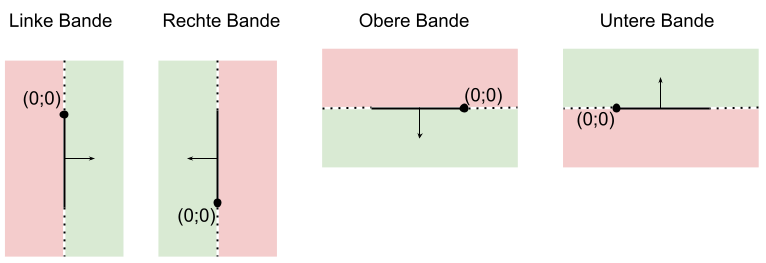
\includegraphics[width=1\linewidth]{../common/03_billiard_ai/resources/49_definitionsbereich_spiegelung_bande.png}
    \end{center}
    \caption{Definitionsbereich einer Bandenspiegelung. Wenn sich ein Zielpunkt im roten Bereich befindet, kann dieser nicht über die Bande angespielt werden.}
    \label{fig:Definitionsbereich_Bandenspiegelung}
\end{figure}

Um für einen Punkt $C$ herauszufinden, ob dieser spiegelbar ist, muss nur geprüft werden, ob er im Definitionsbereich liegt.
Dazu wird der Ursprung des Koordinatensystems zum Start der Bande verschoben und es wird die elementweise Multiplikation
des verschobenen Punktes $C'$ mit der Bandennormale durchgeführt.
Die Elemente des Vektors werden geprüft, ob sie grösser oder gleich dem Nullvektor sind.
Dies resultiert in einem Vektor, welcher eine $0$ speichert, wenn das Element kleiner und $1$, wenn es grösser ist.
Abschliessend wird die quadrierte Länge des resultierenden Vektors gebildet, diese Länge muss $2$ entsprechen, in dem
Fall liegt der Punkt im Definitionsbereich.
\begin{align}
    C^{'} = C \cdot T^0\\
    \bar{C} = C^{'} \cdot \hat{n}\\
    \vec{r} = \bar{C} \geq \vec{0}\\
    l = \vec{r} \cdot \vec{r}\\
    p = l == 2
\end{align}

Wird ein Punkt geprüft, der auf derselben Höhe wie eine Bande liegt, muss zusätzlich die jeweilige Komponente des Punktes
$\bar{C}$ grösser als $0$ sein, bei der die Komponente des Normalenvektors ungleich $0$ ist.

\clearpage
Algorithmus \ref{alg:stoss_ueber_bande_1} und \ref{alg:stoss_ueber_bande_2} zeigt, wie ein Stoss über die Bande gefunden werden kann.
Dazu werden in einem ersten Schritt alle möglichen Kombinationen der Banden gebildet, was auch den letzten Spiegelpunkt
$\bar{C_n}$ generiert. Danach können die Zielpositionen bestimmt werden, wobei auch geprüft wird, ob der Weg zwischen
den Positionen passierbar ist. Sollte dies nicht der Fall sein, wird dieser Lösungskandidat verworfen.

\begin{algorithm}[H]
    \DontPrintSemicolon
    \SetKwFunction{expandByRail}{expandByRail}
    \SetKwFunction{combos}{combos}
    \SetKwFunction{canReflect}{canReflect}
    \SetKwFunction{reflect}{reflect}
    \SetKwProg{Fn}{Function}{}{}
    \Fn{\expandByRail{B: vec2, C: vec2, reflections: int, rails: Rail[]} $\longrightarrow$ Node[]}{
        nodes $\longleftarrow$ Node[]\\
        combinations $\longleftarrow$ combos(reflections, C, rails)\\
        \For{combination in combinations}{
            targets $\longleftarrow$ target(B, C, combination.second,rails, combination.first)\\

            \If{! empty(targets)}{
                nodes $\longleftarrow$ append(physicalEvents(B, C, targets), nodes)
            }
        }
        \KwRet nodes
    }
    \;
    \Fn{\combos{reflections: int, target: vec2, rails: Rail[]} $\longrightarrow$ (Rail[], vec2)[]}{
        combinations: (Rail[], vec2, bool)[] $\longleftarrow$ []\\
        \For{rail in rails}{
            combinations $\longleftarrow$ append(([rail], reflect(target, rail), canReflect(target, rail)), combinations)
        }
        \For{index $\longleftarrow$ 1 < reflections}{
            \For{railIndex $\longleftarrow$ 0 < length(rails)}{
                rail $\longleftarrow$ rails[railIndex]\\
                \If{combinations[railIndex].third and canReflect(combinations[railIndex].second, rail)}{
                    combinations[railIndex].first $\longleftarrow$ append(rail, combinations[railIndex].first)\\
                    combinations[railIndex].second $\longleftarrow$ reflect(combinations[railIndex].second, rail)
                }
                \Else{
                    combinations[railIndex].third $\longleftarrow$ false
                }
            }
        }

        results: (Rail[], vec2)[] $\longleftarrow$ []\\
        \For{railIndex $\longleftarrow$ 0 < length(rails)}{
            \If{combinations[railIndex].third}{
                results $\longleftarrow$ append((combinations[railIndex].first, combinations[railIndex].second), results)
            }
        }

        \KwRet results
    }
    \;
    \Fn{\canReflect{C: vec2, rail: Rail} $\longrightarrow$ bool}{
        moved $\longleftarrow$ C $-$ rail.start\\
        reflected $\longleftarrow$ moved $\cdot$ rail.normal\\
        possible $\longleftarrow$ reflected $\geq \vec{0}$\\
        \KwRet possible $\cdot$ possible $= 2$
    }
    \;
    \Fn{\reflect{C: vec2, rail: Rail} $\longrightarrow$ vec2}{
        reflected: vec3 $\longleftarrow$ vec3(C, 1.0)\\
        \KwRet vec2(rail.M $\cdot$ reflected)
    }
    \caption{Algorithmus zur Berechnung eines Stosses über die Bande - Teil 1}
    \label{alg:stoss_ueber_bande_1}
\end{algorithm}
\newpage
\begin{algorithm}[H]
    \DontPrintSemicolon
    \SetKwFunction{target}{target}
    \SetKwProg{Fn}{Function}{}{}
    \Fn{\target{B: vec2, C: vec2, reflected: vec2, rails: Rail[], combo: Rail[]} $\longrightarrow$ vec2[]}{
        targets $\longleftarrow$ vec2[]\\
        start $\longleftarrow$ B\\
        \While{! empty(combo)}{
            comboRail $\longleftarrow$ pop(combo)\\
            target $\longleftarrow$ $(\infty, \infty)$\\
            \For{rail in rails}{
                railIntersection $\longleftarrow$ halfLineLineSegmentIntersection(start, (reflected - start), rail.start, rail.end)\\
                \If{railIntersection and start <> railIntersection}{
                    target $\longleftarrow$ railIntersection\\
                    reflected $\longleftarrow$ reflect(reflected, rail)\\
                    break
                }
            }
            \If{! shotPossible(start, target)}{
                \KwRet {}
            }
            targets $\longleftarrow$ append(target, targets)\\
            start $\longleftarrow$ target\\
        }

        If{! shotPossible(start, C)}{
            \KwRet {}
        }
        \KwRet targets
    }
    \caption{Algorithmus zur Berechnung eines Stosses über die Bande - Teil 2}
    \label{alg:stoss_ueber_bande_2}
\end{algorithm}

\paragraph{Prüfung der Ausführbarkeit eines Stosses}\mbox{}\\

Für die Expansion einer Kugel, sei es über eine weitere Kugel oder über eine Bande,
muss geprüft werden, dass keine weitere Kugel im Weg ist. Dies wird über die Berechnung
des Distanzvektors zwischen dem Vektor $\vec{d}$ und der zu prüfenden Kugel erzielt. Dasselbe Prinzip wird
in Kapitel \ref{kap:kugelkollision:performanceverbesserung} beim Fall einer dynamisch-statischen Kugelkollision erläutert.

%Bei der Prüfung auf eine mögliche Bandenkollision zwischen der aktuellen Position und dem Zielpunkt muss der Durchmesser
%der Kugel mitberücksichtigt werden. Eine mögliche Situation wird in Abbildung \ref{fig:kugelexpansion_bandenkollision} dargestellt.
%Dazu die Bande $R$ in Normalenrichtung verschoben, wobei die Normale in Richtung des Koordinatenursprungs zeigt. Es resultiert
%die virtuelle Bande $R_V$. Da die Bande durch zwei Punkte (Start und Ende) definiert ist, kann eine Gerade beschrieben werden.
%Dies gilt ebenso für die Kugel $K_1$. Deren Geradengleichung lautet:
%\begin{align}
%    K_1(\lambda) = S - \lambda \cdot \hat{d}
%\end{align}
%Ein Schnittpunkttest zwischen diesen Geraden sollte kein Ergebnis liefern, ansonsten wird vor dem Erreichen des Zielpunkts
%$T$ eine Kollision mit der Bande stattfinden, wie es in diesem Szenario der Fall ist.

%\begin{figure}[h!]
%    \begin{center}
%        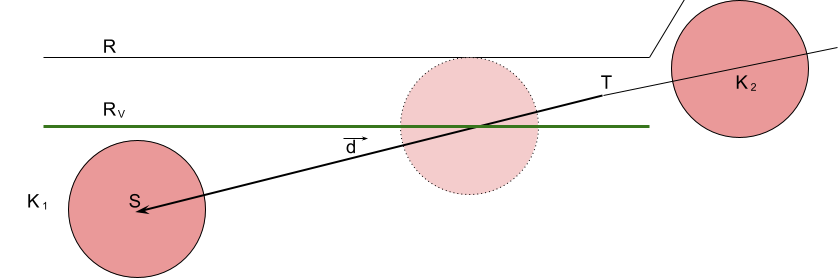
\includegraphics[width=0.5\linewidth]{../common/03_billiard_ai/resources/36_suchkandidat_kugel_expand_banden_kollision.png}
%    \end{center}
%    \caption{Kugelexpansion - Bandenkollision}
%    \label{fig:kugelexpansion_bandenkollision}
%\end{figure}

Sobald die weisse Kugel expandiert wird, muss sichergestellt werden, dass diese auch an der entsprechenden Position
mit dem Queue getroffen werden kann.
Dies wird, wie in Abbildung \ref{fig:kugelexpansion_platz_fuer_queue} veranschaulicht,
durch einen Vektor $\vec{s}$ mit einer bestimmten Länge $s$ entgegen der Rollrichtung der Kugel sowie einem Mindestabstand
$e$ zu diesem Vektor sichergestellt. Die Länge von $e$ wird auf $10 [mm]$ gewählt. Von jeder Kugel aus
werden die Abstände gemessen, liegt die Kugel zwischen $W$ und $W + \vec{s}$, so wird der Abstand senkrecht zum Vektor $\vec{s}$
berechnet, zu sehen bei der Kugel $K_1$. Liegt die Kugel wie $K_2$ vorne oder hinten, wird der Abstand zum Punkt $W$ oder $W + \vec{s}$
berechnet. Für die so erhaltenen Distanzen $d_i$ muss gelten, wobei $r$ für den Kugelradius steht:
\begin{align}
    d_i >= e + r
\end{align}

Liegt die Kugel in Richtung der Rollrichtung, wurde die Bedingung bereits geprüft, ansonsten dürfte die weisse Kugel nicht
expandiert worden sein. Daher muss dieser Fall nicht speziell behandelt werden.

\begin{figure}[h!]
    \begin{center}
        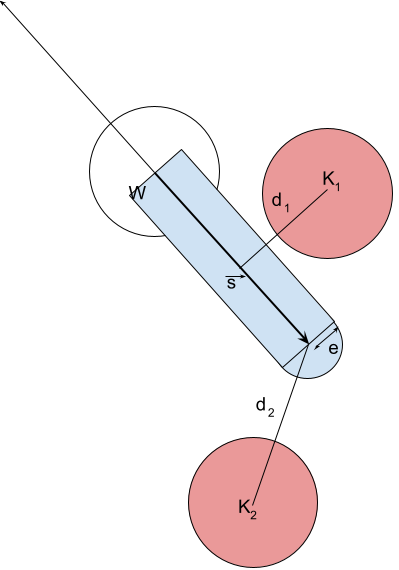
\includegraphics[width=0.3\linewidth]{../common/03_billiard_ai/resources/37_platz_fuer_queue.png}
    \end{center}
    \caption{Kugelexpansion - Platz für Queue. Der blau hinterlegte Bereich hinter der weissen Kugel darf nicht von anderen Kugeln belegt sein,
        damit diese mithilfe des Queues wie gewünscht angestossen werden kann.}
    \label{fig:kugelexpansion_platz_fuer_queue}
\end{figure}

\newpage
\subsubsection{Bewertungsfunktion}
Um die Suche zu vereinfachen und in eine spezifische Richtung zu lenken, wo die besten Resultate zu erwarten sind, ist
es unerlässlich eine Bewertung des Stosses durchzuführen.
Die Bewertungsfunktion wurde so definiert, dass sie sich auf den aktuell expandierten Knoten beschränkt.
Die Kosten für eine Expansion werden über die Pfade aufsummiert.
Anhand der Summen kann jeweils der kostengünstigste Pfad evaluiert und verfolgt werden.
Abbildung \ref{fig:suchbaum_bewertung} zeigt das Prinzip.
Dieses Vorgehen entspricht demjenigen des Dijkstra-Algorithmus \cite{wiki.dijkstra:1}.
\begin{figure}[h!]
    \begin{center}
        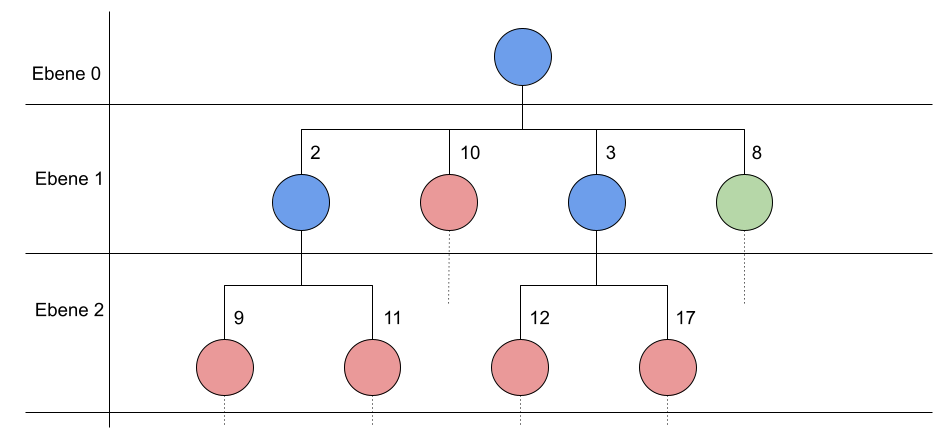
\includegraphics[width=0.8\linewidth]{../common/03_billiard_ai/resources/28_suchbaum_bewertung.png}
    \end{center}
    \caption{Bewertung eines Suchbaums: Die Knoten werden je nach Bedeutung mit unterschiedlichen Farben markiert.
    Wenn sie bereits expandiert wurden, sind sie blau. Grün, wenn der Knoten im nächsten Schritt expandiert wird,
    da er die geringsten Pfadkosten aufweist und rot, wenn der Knoten nicht in Frage kommt aufgrund zu hoher Kosten.}
    \label{fig:suchbaum_bewertung}
\end{figure}

Die Kosten werden auf Basis dreier Kriterien\footnote{Die Kriterien Distanz und Winkel werden wie
in Publikation \cite{inproceedings:billiard_ai:1} verwendet.} gebildet:
\begin{enumerate}
    \item Die \emph{Distanz}, welche eine Kugel zurücklegt.
    \item Der \emph{Winkel}, in welcher ein Zielpunkt getroffen werden muss.
    \item Die \emph{Indirektion}, wenn eine Kugel über die Banden oder über eine andere Kugel angestossen wird.
\end{enumerate}

Jeder dieser Werte liegt zwischen $0$ und $1$.
Die ersten beiden Kriterien sind in Abbildung \ref{fig:suche_knoten_expansionskosten} dargestellt.
Es werden zwei Expansionen gezeigt.
Die relevanten Informationen $d$ für die Distanz sowie $\alpha$ für den Winkel weisen
einen entsprechenden Index auf, welcher den Expansionsschritt markiert.
Beim ersten Expansionsschritt bildet der Zielpunkt
den Elternknoten.
Der Winkel $\alpha_1$ ist definiert durch die Rollrichtung der Kugel und einer Normalen auf den Zielpunkt.
Die Normalen zeigen jeweils zum Ursprung in der Mitte des Tisches.
Die Distanz $d_1$ ist definiert über die Länge des zurückzulegenden Weges.
Ist in einem Expansionsschritt die weisse Kugel betroffen, werden die Distanzkosten mit den
Distanzkosten des vorangegangenen Expansionsschritts gewichtet.
Dies stellt sicher, dass der Weg, welcher die nächste Kugel nehmen wird, möglichst kurz sein muss,
damit sich ein allfälliger Fehler beim Stoss der weissen Kugel nicht zu stark akkumuliert.
Im zweiten Fall wird der Winkel $\alpha_2$ durch die Rollrichtung der ersten und der Rollrichtung der zweiten Kugel definiert.

\begin{figure}[h!]
    \begin{center}
        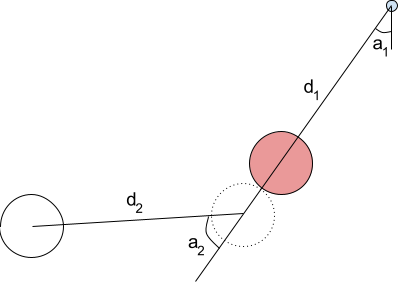
\includegraphics[width=0.4\linewidth]{../common/03_billiard_ai/resources/29_suchbaum_expansionskosten.png}
    \end{center}
    \caption{Zusammensetzung der Kosten eines Stosses:
    Die Kugeln müssen die Distanzen $d_1$ und $d_2$ zurücklegen.
    Die rote Kugel muss im Winkel $\alpha_1$ getroffen werden.
    Die rote Kugel wird dadurch im Winkel $\alpha_2$ in das Zielloch gespielt.
    Der Vektor $\vec{n}$ ist die Normale des Ziellochs, welche für die Berechnung des Winkels $\alpha_2$ verwendet wird.
    }
    \label{fig:suche_knoten_expansionskosten}
\end{figure}

Um die beiden Grössen vergleichen zu können, müssen sie in dieselbe Grössenordnung gebracht werden. Aus diesem Grund
werden sie durch die maximal möglichen Werte normiert \cite{qucosa:ein_billardroboter:1}. Für die Distanz ist dies die
Diagonale über den Tisch, für den Winkel wird ein maximal möglicher Wert von $87^\circ$ gewählt, dies ist bereits bei
der Suche berücksichtigt. Es gilt die Annahme, dass je kürzer der Weg und je kleiner der Winkel,
desto einfacher der Stoss.
\begin{align}
    d_{krit} = \frac{d_i}{d_{max}}\\
    \alpha_{krit} = \frac{\alpha}{\alpha_{max}}
\end{align}
Aktuell fliesst der Winkel $\alpha_{krit}$ zu stark in die Bewertung ein. Daher wird dieser durch eine kubische
Bézier-Kurve \cite{wiki.bezier:1} gewichtet. Die Parameter lauten wie folgt.
\begin{align}
    P_0 = \begin{pmatrix} 0 & 0\end{pmatrix}\\
    P_1 = \begin{pmatrix} 1 & 0\end{pmatrix}\\
    P_2 = \begin{pmatrix} 0.5 & 1\end{pmatrix}\\
    P_3 = \begin{pmatrix} 1 & 1\end{pmatrix}\\
    P = \begin{pmatrix} P_0 \\ P_1 \\ P_2 \\ P_3\end{pmatrix}\\
    T = \begin{pmatrix} t^3 & t^2 & t & 1\end{pmatrix}\\
    M = \begin{pmatrix}
            -1 &  3 & -3 & 1\\
             3 & -6 &  3 & 0\\
            -3 &  3 &  0 & 0\\
             1 &  0 &  0 & 0
        \end{pmatrix}\\
    \alpha^G_{krit} = f(t = \alpha_{krit}) = T \cdot M \cdot P
\end{align}
Nach dieser Gewichtung resultiert ein Punkt im zweidimensionalen Raum, wovon die y-Komponente als $\alpha^G_{krit, y}$ verwendet wird.
Die Kurve ist in Abbildung \ref{fig:suche_knoten_gewichtung_winkelkosten}
visualisiert. Es wird deutlich, dass kleinere Winkel einen eher geringen Einfluss auf die Kosten haben.
Ab einem Winkel von $50^\circ$, welcher auf der Grafik \ref{fig:suche_knoten_gewichtung_winkelkosten} als Punkt $D_1$ markiert ist,
beginnt die Kurve bis etwa $80^\circ$ stark zu steigen.
Ab dort flacht sie wiederum ab, bis die Kosten von $90^\circ$ schliesslich den Wert $1$ erreichen.

\begin{figure}[h!]
    \begin{center}
        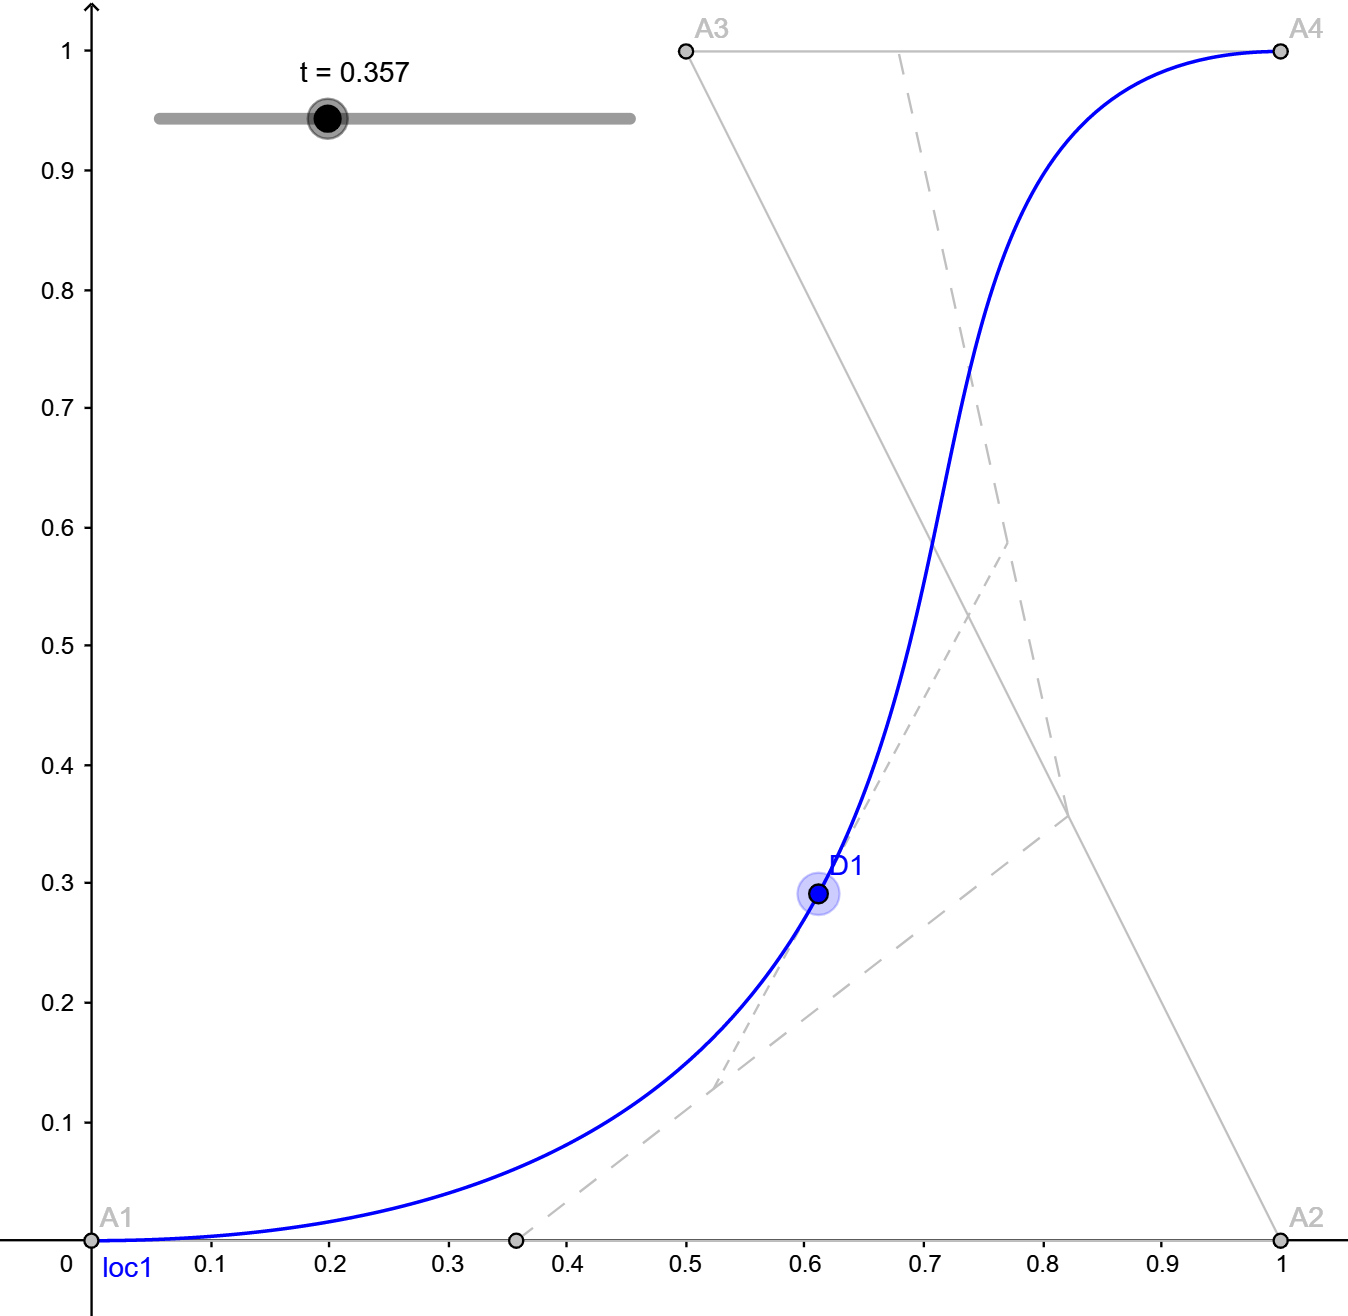
\includegraphics[width=0.4\linewidth]{../common/03_billiard_ai/resources/30_suchbaum_gewichtung_winkelkosten.png}
    \end{center}
    \caption{Gewichtung der Winkelkosten mittels einer Bézier-Kurve.
    Kleine Winkel werden in den Kosten geringer gewichtet, während grosse Winkel eine höhere Gewichtung erhalten.}
    \label{fig:suche_knoten_gewichtung_winkelkosten}
\end{figure}

Das Kriterium der Indirektion über Kugeln wird wiederum über einen maximal möglichen Wert gelöst.
Es wird eine maximale Indirektion $K_{I,max}$ angegeben und die Anzahl der Vorkommnisse ${K_{I,n}}$ wird durch die
Konstante dividiert. Dadurch werden die Kosten erhöht, je grösser der Indirektionsgrad ist.
\begin{align}
    K_{I,krit} = \frac{K_{I,n}}{K_{I,max}}
\end{align}

Das Kriterium der Indirektion über Banden wird ebenso über einen maximal möglichen Wert gelöst.
Es wird eine maximale Indirektion $K_{B,max}$ angegeben und die Anzahl der Vorkomnisse ${K_{B,n}}$ wird durch die
Konstante dividiert. Dadurch werden die Kosten erhöht, je grösser der Indirektionsgrad ist.
\begin{align}
    K_{B,krit} = \frac{K_{B,n}}{K_{B,max}}
\end{align}

Die endgültigen Kosten werden über die Addition aller Kriterien gebildet.
\begin{align}
    K = d_{krit} + \alpha^G_{krit, y} + K_{I,krit} + K_{B,krit}
\end{align}

